\section{Additional results and details}
\subsection{Search procedures and reporting-method details}
\emph{Random search} (RS, budget $B$): $B$ distinct configurations drawn uniformly from the pool, all evaluated on all of $S$, argmax (random tie-break). \emph{Successive halving}: $B$ random candidates, reduction factor 3, rungs evaluated on nested random subsets of $S$ of size $n/3^{r}$ (at least 25), the last rung on all of $S$, winner = best on the last rung. \emph{Coordinate ascent}: random start, then up to two passes over the three factors (format$\times$demonstrations, instruction, cue) in random order, each time evaluating all levels of one factor on all of $S$ and moving to the best (about 26 evaluations). \emph{MIPRO-like}: 40 trials; a trial samples each factor level either uniformly (probability 0.3 or first two trials) or from a softmax (temperature 0.03) over the running mean minibatch score of the levels, evaluates the sampled configuration on a random minibatch of 50 items of $S$, then the 3 configurations with the highest average minibatch score are evaluated on all of $S$ and the best is returned. Reports are always the winner's score on all of $S$.
\emph{Hold-out}: random 30\% of $S$ held out; search on the remaining 70\%. \emph{Cross-fit}: 5 random folds; interval = Wald on pooled held-out outcomes. \emph{Replay bootstrap}: 100 resamples (with replacement) of $S$, the whole search (including its internal randomness) re-run on each; interval = corrected point estimate $\pm1.96\sqrt{\hat p(1-\hat p)/n}$. \emph{EB}: interval = estimate $\pm1.96\sqrt{\kappa\hat\sigma^2+\hat s_m^2}$, $\hat s_m^2$ the sampling variance of the grand mean over items (accounts for shared item noise). \emph{Conditional}: polyhedral truncated-normal CI inverted by root-finding, covariance from the item-level matrix. \emph{Simultaneous}: 500 bootstrap draws of the max-$t$ statistic. \emph{Ladder}: step $\eta=n^{-1/2}$, reported = rounded best. \emph{Thresholdout}: $S$ split in halves; threshold $T$ and Laplace noise scale $\sigma_T$ as multiples of the SE of the difference of half-sample accuracies (main setting $T{=}1\cdot$SE, $\sigma_T{=}0.1\cdot$SE; two other settings were also tried and were no better).

\subsection{Optimism of the status-quo report on the real pool}
\begin{table}[h]
\centering\small
\caption{Reported minus true accuracy of the selected configuration (pts, $\pm1.96$ MC SE), real pool, benchmark of $n$ questions drawn i.i.d.\ from the cached population; 400 draws per cell.}
\label{tab:realopt}
\begin{tabular}{lccccc}
\toprule
 & $n{=}50$ & 100 & 200 & 400 & 800 \\
\midrule
RS $B{=}8$ & 5.0$\pm$0.6 & 3.3$\pm$0.4 & 2.2$\pm$0.3 & 1.3$\pm$0.2 & 0.8$\pm$0.2 \\
RS $B{=}72$ & 7.8$\pm$0.6 & 5.4$\pm$0.4 & 3.7$\pm$0.3 & 2.3$\pm$0.2 & 1.2$\pm$0.1 \\
SH $B{=}72$ & 5.5$\pm$0.6 & 3.2$\pm$0.4 & 1.7$\pm$0.3 & 1.2$\pm$0.2 & 0.8$\pm$0.2 \\
coord.\ asc. & 6.4$\pm$0.6 & 4.4$\pm$0.4 & 3.0$\pm$0.3 & 2.0$\pm$0.2 & 1.2$\pm$0.1 \\
MIPRO-like & 7.2$\pm$0.6 & 3.7$\pm$0.4 & 2.1$\pm$0.3 & 1.5$\pm$0.2 & 0.8$\pm$0.1 \\
\bottomrule
\end{tabular}

\end{table}

\subsection{Reporting methods: numbers}
\begin{table}[h]
\centering\small
\caption{Synthetic worlds ($\rho{=}0.8$; $\tau$ in probit units; 300 draws per cell). Entries: bias / RMSE (pts) / coverage (\%) for the accuracy of the deployed configuration.}
\label{tab:synthmeth}
\resizebox{\linewidth}{!}{\begin{tabular}{lcccc}
\toprule
setting & naive & hold-out & cross-fit & replay-boot. \\
\midrule
$\tau{=}0.0$, RS $B{=}72$, $n{=}100$ & +7.6/8.5/76 & +0.2/9.5/91 & -0.0/5.7/92 & +2.5/4.8/95 \\
$\tau{=}0.0$, RS $B{=}72$, $n{=}400$ & +3.8/4.3/65 & -0.3/4.3/94 & -0.2/2.8/92 & +1.1/2.3/99 \\
$\tau{=}0.0$, MIPRO-like, $n{=}100$ & +5.6/7.0/86 & -0.2/8.6/96 & +0.2/4.7/97 & +1.6/4.6/97 \\
$\tau{=}0.0$, MIPRO-like, $n{=}400$ & +2.1/3.0/88 & +0.5/4.3/94 & +0.4/2.4/96 & +0.6/2.2/97 \\
$\tau{=}0.1$, RS $B{=}72$, $n{=}100$ & +5.6/7.4/80 & +0.5/9.1/95 & +0.1/6.6/82 & +1.4/5.3/94 \\
$\tau{=}0.1$, RS $B{=}72$, $n{=}400$ & +1.7/2.7/95 & -0.1/4.7/94 & -0.2/2.9/94 & +0.1/2.3/97 \\
$\tau{=}0.1$, MIPRO-like, $n{=}100$ & +4.4/6.3/88 & +1.1/8.6/96 & +0.1/5.8/91 & +1.0/4.8/96 \\
$\tau{=}0.1$, MIPRO-like, $n{=}400$ & +1.1/2.5/95 & +0.2/4.1/96 & +0.1/3.3/87 & +0.0/2.3/97 \\
\bottomrule
\end{tabular}
}
\end{table}
\begin{table}[h]
\centering\small
\caption{Real pool, random search $B{=}72$ evaluated exhaustively on $S$: bias / RMSE / coverage (\%) / median interval width (pts). Conditional: median-unbiased estimator is unbounded in a sizeable fraction of draws, so only coverage and width are given.}
\label{tab:extras}
\resizebox{\linewidth}{!}{\begin{tabular}{lccccccc}
\toprule
 & naive & EB shrink & worst-case corr. & conditional & simultaneous & Ladder & Thresholdout \\
\midrule
RS $B{=}72$, $n{=}100$ & +5.4/6.8/86/19 & +0.0/4.0/94/15 & -0.8/4.0/98/19 & --/--/97/30 & +5.4/6.8/98/28 & +1.4/4.8/91/20 & +9.9/11.0/78/28 \\
RS $B{=}72$, $n{=}400$ & +2.1/3.0/89/9 & -0.3/2.2/90/8 & -1.0/2.4/94/9 & --/--/97/15 & +2.1/3.0/99/14 & +1.0/2.6/94/10 & +4.6/5.2/86/14 \\
\bottomrule
\end{tabular}
}
\end{table}
\begin{table}[h]
\centering\small
\caption{Robustness to the shape of the candidate-quality distribution (synthetic, $K{=}72$ i.i.d.\ configuration effects, true SD $\tau{=}0.05$ probit units, $n{=}100$, 200 draws): bias (pts) / coverage (\%).}
\label{tab:robust}
\resizebox{\linewidth}{!}{\begin{tabular}{lccccccc}
\toprule
 config.\ effects & naive & replay-boot. & hold-out & EB & worst-case & conditional & simult. \\
\midrule
normal & +6.8/77 & +2.0/94 & -0.5/96 & +0.2/96 & -0.5/98 & --/96 & +6.8/98 \\
sparse & +3.9/89 & -0.3/95 & -0.2/94 & -4.1/74 & -3.3/90 & --/94 & +4.0/98 \\
heavy & +5.5/82 & +0.6/92 & -0.5/95 & -0.9/87 & -1.5/94 & --/95 & +5.8/98 \\
bimodal & +6.4/80 & +1.5/97 & +0.2/95 & +1.5/97 & -0.8/98 & --/97 & +6.6/98 \\
\bottomrule
\end{tabular}
}
\end{table}

\begin{figure}[h]
\centering
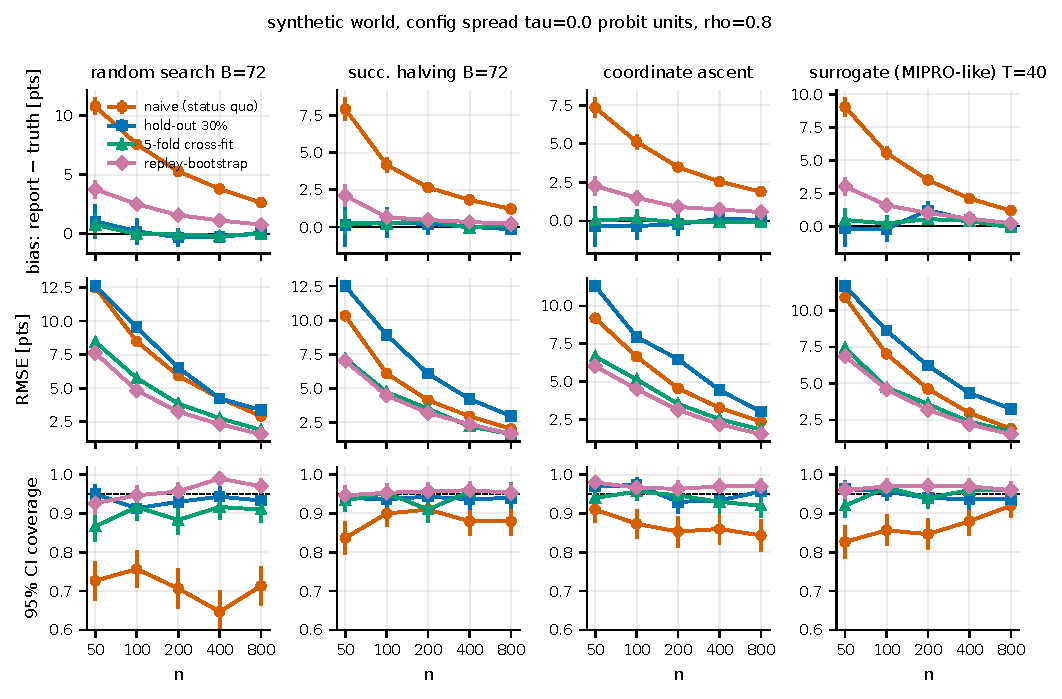
\includegraphics[width=\linewidth]{figs/fig_methods_synth_tau00.pdf}\\
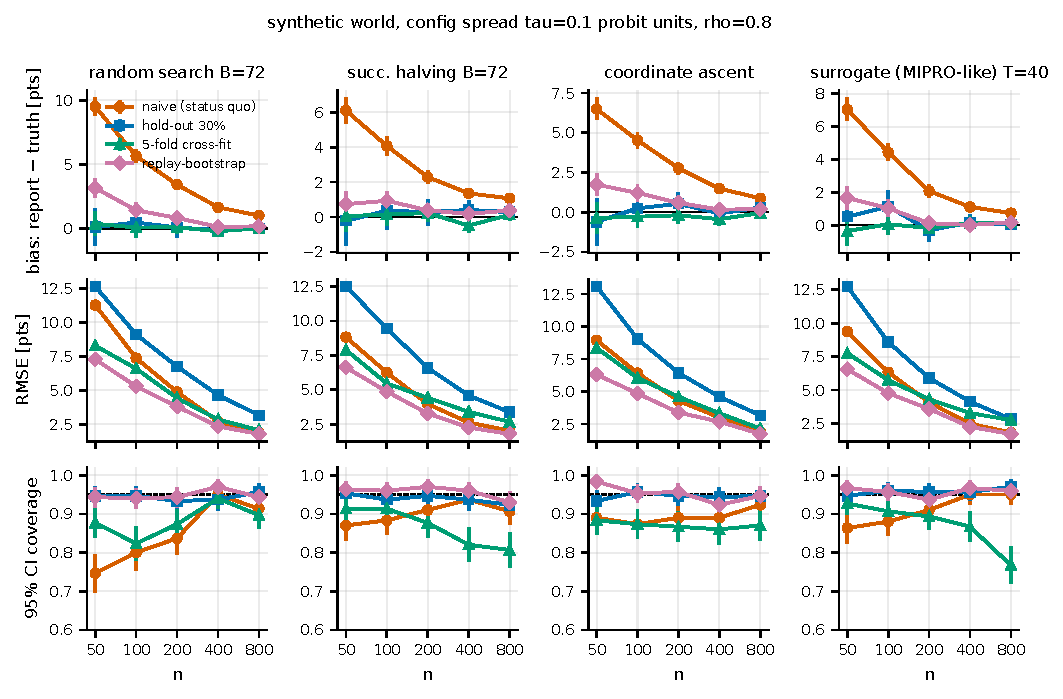
\includegraphics[width=\linewidth]{figs/fig_methods_synth_tau10.pdf}
\caption{Synthetic counterpart of Fig.~\ref{fig:methods}: configuration spread $\tau{=}0$ (top) and $\tau{=}0.1$ probit units (bottom), $\rho{=}0.8$, 300 draws per cell.}
\label{fig:methods_synth}
\end{figure}

\subsection{Number of bootstrap replays}
\label{app:boot}
\begin{table}[h]
\centering\small
\caption{Replay bootstrap, real pool, $n{=}100$: bias / RMSE (pts) / coverage (\%) of the corrected report as a function of the number of replays $b$ (300 benchmark draws per cell).}
\begin{tabular}{lcccc}
\toprule
 & $b{=}10$ & 25 & 100 & 300 \\
\midrule
RS $B{=}72$ & +1.6 / 4.5 / 96 & +1.5 / 4.7 / 95 & +1.4 / 4.4 / 96 & +0.9 / 4.4 / 96 \\
MIPRO-like & +1.4 / 4.7 / 94 & +0.8 / 4.3 / 96 & +0.8 / 4.2 / 98 & +1.1 / 4.0 / 97 \\
\bottomrule
\end{tabular}

\end{table}

\subsection{Label-permutation negative control}
\begin{table}[h]
\centering\small
\caption{Optimism (pts) of the status-quo report with real gold labels / with permuted gold labels (all configurations then at chance, accuracy about \PermAcc\%), same search procedures and benchmark draws (300 draws per cell, benchmarks drawn i.i.d.\ from the cached population).}
\label{tab:permnull}
\begin{tabular}{lccccc}
\toprule
 & $n{=}50$ & 100 & 200 & 400 & 800 \\
\midrule
RS $B{=}8$ & 5.0 / 4.3 & 3.3 / 2.7 & 2.5 / 2.0 & 1.5 / 1.2 & 0.9 / 0.8 \\
RS $B{=}72$ & 8.0 / 6.5 & 5.6 / 4.8 & 3.6 / 3.1 & 2.1 / 2.1 & 1.2 / 1.2 \\
SH $B{=}72$ & 5.8 / 4.2 & 3.0 / 2.6 & 1.7 / 1.6 & 1.2 / 1.0 & 0.8 / 0.7 \\
coord.\ asc. & 7.6 / 4.9 & 4.7 / 3.7 & 2.9 / 2.4 & 2.0 / 1.5 & 1.0 / 1.0 \\
MIPRO-like & 7.6 / 5.9 & 4.4 / 3.5 & 2.3 / 2.0 & 1.5 / 1.1 & 0.7 / 0.6 \\
\bottomrule
\end{tabular}

\end{table}

\subsection{Why the primary real analysis draws benchmarks with replacement}
\label{app:wr}
If $S$ is drawn without replacement from a finite pool $P$ of $N$ questions and truth is taken as the accuracy on the remaining $N-n$ questions, then for any fixed configuration $\mathrm{fresh}=\bar y_P-\frac{n}{N-n}(\bar y_S-\bar y_P)$: the fresh accuracy is mechanically anti-correlated with the benchmark accuracy, and the measured optimism is inflated by the factor $N/(N-n)$ relative to its value for a benchmark drawn from the population $P$ itself. With $N=\RealN$ the factor is \PoolFactorNHund\ at $n{=}100$ and $1.67$ at $n{=}400$. We therefore draw $S$ i.i.d.\ from $P$ (with replacement) and use the exact accuracy over $P$ as truth. As a check, for $n\le200$ where the inflation is small, benchmarks drawn without replacement and scored on $P\setminus S$ give naive / replay-bootstrap / hold-out biases of \FreshNaiveRSNFifty/\FreshBootRSNFifty/\FreshHoldRSNFifty\ ($n{=}50$), \FreshNaiveRSNHund/\FreshBootRSNHund/\FreshHoldRSNHund\ ($n{=}100$) and \FreshNaiveRSNTwoH/\FreshBootRSNTwoH/\FreshHoldRSNTwoH\ ($n{=}200$) pts for RS $B{=}72$, versus \NaiveRSNFifty/\BootRSNFifty/\HoldRSNFifty, \NaiveRSNHund/\BootRSNHund/\HoldRSNHund\ and \NaiveRSNTwoH/\BootRSNTwoH/\HoldRSNTwoH\ with the primary design; the qualitative picture is unchanged.

\subsection{Derivation of eq.~\eqref{eq:opt}}
\label{app:proof}
Let $\mu_c\sim\mathcal N(m,\tau^2)$, $\varepsilon_c\sim\mathcal N(0,\sigma^2)$ independent over $c=1..B$, $\bar Y_c=\mu_c+\varepsilon_c$, $\hat c=\arg\max_c\bar Y_c$. The $\bar Y_c$ are i.i.d.\ $\mathcal N(m,\tau^2+\sigma^2)$, so $\bar Y_{\hat c}=m+\sqrt{\tau^2+\sigma^2}\,Z_{(B)}$ with $Z_{(B)}$ the maximum of $B$ standard normals, independent of nothing else needed. By normal-normal conjugacy $\mathbb{E}[\mu_c\mid\bar Y_1..\bar Y_B]=m+\kappa(\bar Y_c-m)$ with $\kappa=\tau^2/(\tau^2+\sigma^2)$, and this holds also at the random index $\hat c$, because $\hat c$ is a function of $(\bar Y_c)_c$. Hence $\mathbb{E}[\mu_{\hat c}-m]=\kappa\sqrt{\tau^2+\sigma^2}\,\mathbb{E}Z_{(B)}$ and $\mathbb{E}[\bar Y_{\hat c}-\mu_{\hat c}]=(1-\kappa)\sqrt{\tau^2+\sigma^2}\,\mathbb{E}Z_{(B)}=\sigma^2(\tau^2+\sigma^2)^{-1/2}\mathbb{E}Z_{(B)}$. Without the prior: for any fixed $\mu$, $\mathbb{E}[\max_c\varepsilon_c]\le\sigma\sqrt{2\ln B}$ and $\max_c\bar Y_c-\mu_{\hat c}\le\max_c\varepsilon_c$, so the optimism is at most $\sigma\sqrt{2\ln B}$. For binary scores on shared items, $\sigma^2$ is the variance of the configuration-specific part of the accuracy, $\approx(1-\bar r)p(1-p)/n$; in the simulations of Fig.~\ref{fig:theory} it is measured from the data. The formula is exact only under the stated Gaussian i.i.d.\ structure and ignores ties and the discreteness of accuracies.

\subsection{Compute actually used}
All experiments ran on a 4-core CPU quota (no GPU). Real-LLM scoring: one forward pass per (question, prompt prefix) plus short suffix passes with KV-cache reuse: $\RealN{\times}72$ cached score vectors for Qwen2.5-1.5B-Instruct (8-bit GGUF) took about 16 wall-clock hours on 3--4 cores, plus the Real-II grids (App.~\ref{app:real2}) and the demonstration-leak check (about 1.5 h on one core). All statistical Monte-Carlo (synthetic: about 6 CPU-hours in total; real replays: about 1 CPU-hour) ran on the cached scores.

\subsection{Real-II: a pool with true signal (model $\times$ prompt)}
\label{app:real2}
Pool: Qwen2.5-1.5B (from the main grid, the 8 matching configurations), Qwen2-1.5B, Qwen3-1.7B (non-thinking mode: empty think block in the assistant turn) and Qwen3-0.6B, 8-bit GGUF, each with the two groups \{zero-shot, 3-shot set 1\} $\times$ instructions \{0,1\} $\times$ cues \{0,1\} of the main grid, scored by the same next-token-letter rule on the first 250 questions of the item permutation (10 chunks of 25 questions; the plan of 24 chunks and a fifth model, Qwen2.5-0.5B, was cut for compute). Benchmarks of $n\in\{50,100,200\}$ are drawn i.i.d.\ from these 250 questions (with $n{=}200$ most draws contain many duplicates, so that column is least reliable), truth = accuracy over the 250. Random search with $B{=}8$ or $B{=}K{=}32$ and successive halving ($B{=}32$) were replayed (coordinate ascent and the MIPRO-like search use the factor structure of the main grid and are not applicable).
\begin{figure}[h]
\centering
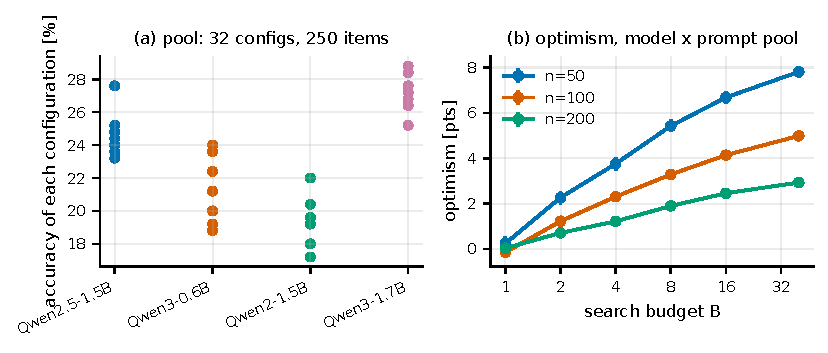
\includegraphics[width=0.75\linewidth]{figs/fig_real2.pdf}
\caption{Real-II pool: (a) population accuracy of each configuration by model; (b) optimism of the naive report vs.\ search budget (400 draws per $n$, $\pm1.96$ SE).}
\end{figure}
\begin{table}[h]
\centering\small
\caption{Real-II, random search over all 32 configurations: bias (pts) / RMSE / coverage (\%) by reporting method.}
\begin{tabular}{lcccc}
\toprule
 & naive & hold-out & cross-fit & replay-boot. \\
\midrule
$n{=}50$ & +7.5/9.2/87 & -1.3/11.2/96 & -1.2/7.9/84 & +1.5/6.1/96 \\
$n{=}100$ & +4.8/6.2/88 & -0.4/8.0/97 & -0.4/5.9/84 & +0.8/4.5/93 \\
$n{=}200$ & +2.9/4.0/89 & +0.1/5.9/96 & -0.0/4.1/86 & +0.5/3.2/95 \\
\bottomrule
\end{tabular}

\end{table}
